\documentclass{beamer}

\usepackage{listings}  % Package to include python syntax code
\usepackage{color} % Package to include colors for syntax highlighting
\usepackage{graphicx}  % Package to include images
\usepackage{hyperref}  % Hyperlinks
\usepackage{tikz}

\lstset{  % Settings for listings package
backgroundcolor=\color{cyan!10},  % Includes a light blue background color
numbers=left,  % Includes line numbers
keywordstyle=\bfseries\color{green!40!black},  % Bold and color green for keywords
identifierstyle=\color{blue},  % Other words are colored blue
stringstyle=\color{orange},  % Strings are orange
showstringspaces=false  % Don't show spaces in strings
}

\setbeamertemplate{navigation symbols}{}  % Remove navigation symbols

\title{Computing for Mathematics: Week 1}
\date{}


\begin{document}

\frame{
\titlepage
}

\frame{
\frametitle{Vince Knight}

\begin{itemize}
    \item Office: M1.25
    \item email: knightva@cf.ac.uk
    \item Office hours: Thursday 1300 - 1500
\end{itemize}

}

\frame{
\href{https://www.youtube.com/watch?v=qEr6mcgdsmI}{
$$\begin{pmatrix}
(0,0) & (-1,1) & (1,-1)\\
(1,-1) & (0,0) & (-1,1)\\
(1,-1) & (-1,1) & (0,0)\\
\end{pmatrix}$$}
}

\frame{
\frametitle{Programming and Mathematics}

There are various areas in which computers are of major importance to Mathematicians:

\begin{itemize}
\item Computer assisted proofs;
\item Implementation of mathematics;
\item Computer generated proofs;
\item Everyday mathematics.
\end{itemize}

}

\frame{
\frametitle{Computer assisted proofs}

\begin{center}

\begin{tikzpicture}

\only<1>{
\node (A) [circle, draw] at (-.5,2) {0};
\node (B) [circle, draw] at (0,1) {1};
\node (C) [circle, draw] at (1.5,2) {2};
\node (D) [circle, draw] at (-.5,0) {3};
\node (E) [circle, draw] at (2,.7) {4};
}

\only<2>{
\node (A) [circle, draw, fill=blue] at (-.5,2) {0};
\node (B) [circle, draw] at (0,1) {1};
\node (C) [circle, draw] at (1.5,2) {2};
\node (D) [circle, draw] at (-.5,0) {3};
\node (E) [circle, draw] at (2,.7) {4};
}

\only<3>{
\node (A) [circle, draw, fill=blue] at (-.5,2) {0};
\node (B) [circle, draw, fill=green] at (0,1) {1};
\node (C) [circle, draw] at (1.5,2) {2};
\node (D) [circle, draw] at (-.5,0) {3};
\node (E) [circle, draw] at (2,.7) {4};
}

\only<4>{
\node (A) [circle, draw, fill=blue] at (-.5,2) {0};
\node (B) [circle, draw, fill=green] at (0,1) {1};
\node (C) [circle, draw, fill=red] at (1.5,2) {2};
\node (D) [circle, draw, fill=red] at (-.5,0) {3};
\node (E) [circle, draw] at (2,.7) {4};
}

\only<5-6>{
\node (A) [circle, draw, fill=blue] at (-.5,2) {0};
\node (B) [circle, draw, fill=green] at (0,1) {1};
\node (C) [circle, draw, fill=red] at (1.5,2) {2};
\node (D) [circle, draw, fill=red] at (-.5,0) {3};
\node (E) [circle, draw, fill=gray] at (2,.7) {4};
}
\draw (A) -- (C);
\draw (A) -- (B);
\draw (A) -- (D);
\draw (A) -- (E);
\draw (B) -- (C);
\draw (B) -- (E);
\draw (B) -- (D);
\draw (E) -- (D);
\draw (E) -- (C);
\end{tikzpicture}
\end{center}

\begin{itemize}
\onslide<5-6>{
\item `4 colour theorem': \textbf{Any map can be coloured using 4 colours.\\}
}

\onslide<6>{

\item Proved in 1976 by Kenneth Appel and Wolfgang Haken:
\begin{center}
\framebox{Used computers to check 1936 particular cases.}
\end{center}
}
\end{itemize}
}

\frame{
\frametitle{Computer assisted proofs}
Slide about sphere packing problem.
}

\frame{
\frametitle{Implementation of mathematics}
Show Leanne's model
}

\frame{
\frametitle{Computer generated proofs}
Show a computer generated proof
}

\frame{
\frametitle{Everyday mathematics}
Show a simple integral
}

\frame{
\frametitle{Flipped classrooms}
\pause
\begin{center}
    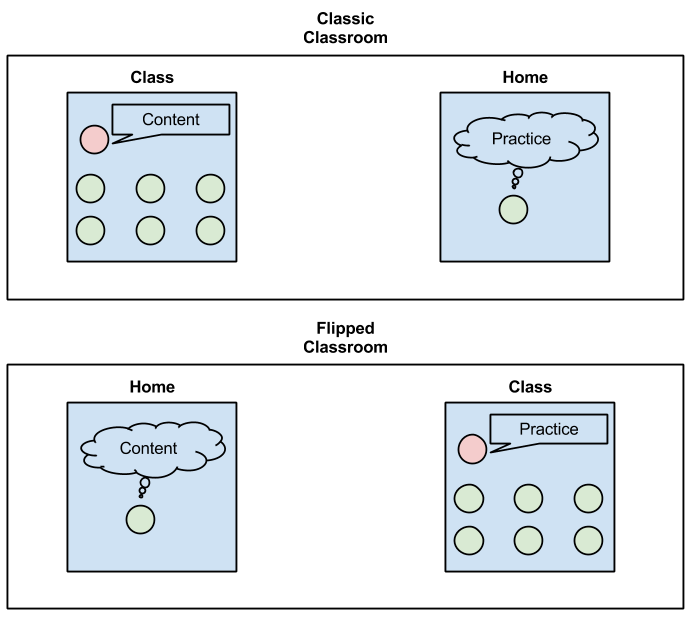
\includegraphics[width=8cm]{./images/W01-img01.png}
\end{center}
}

\frame{
\frametitle{`Tickables'}
Include bullet points
}

\frame{
\frametitle{Resources}
Show resources.
}

\begin{frame}[fragile]
\frametitle{Some code}

Here is some example code:

\begin{lstlisting}[language=python]
for i in range(10):
    print 'The number is: ',i
\end{lstlisting}

\end{frame}

\end{document}
